%DO NOT MESS AROUND WITH THE CODE ON THIS PAGE UNLESS YOU %REALLY KNOW WHAT YOU ARE DOING
\chapter*{Experimental Research}
\addcontentsline{toc}{chapter}{Experimental Research}


\section{ Pressure distribution } \label{ Pressure distribution } 
\noindent The MATLAB program for determining the pressure distribution was developed. The following parameter values were considered.
\begin{center}
\begin{tabular}{ |c|c| } 
 \hline
 \multicolumn{2}{|c|}{Signal Parameters} \\
 \hline
  Waveform type & Sinusoidal \\
  Amplitude, \textit{A} & 1\\ 
  Frequency, \textit{f} & 10 Hz, 100 Hz, 1 kHz, 10 kHz and 100 kHz  \\ 
   \hline
\end{tabular}
\end{center}

\begin{center}
\begin{tabular}{ |c|c| } 
 \hline
 \multicolumn{2}{|c|}{Waveguide Parameters} \\
 \hline
  Water depth, \textit{D} & 20 m \\
  Source location & \textit{$r_{S}$} = 0 m and \textit{$z_{S}$} = 5 m \\ 
  Receiver location & $(r_{R},z_{R})^{T} \in [0, 500] \times [0, \textit{D}] $\\ 
  Bottom type & Hard, i.e. $ \textit{$R_{2}$} = 1$ \\
  Sound speed, \textit{c} & 1480 m/s \\
   \hline
\end{tabular}
\end{center}

\newpage

\noindent The pressure distribution is a function of source location, receiver location and angular frequency. For the given point source coordinates $(0, z_{S})$ the pressure shall be determined at an arbitrary receiver location $(r_{R}, z_{R}).$ More the pressure value, better is the prorogation of sound as hydrophones work on the phenomenon of pressure variation. 

\noindent At low frequencies, when the transmission is close to the horizontal,  sound wave reflection yields an interesting effect because the reflected signal interferes with the direct path signal. The coherent summation of two signals produces the spatial interference fringes. When the frequency is 10 Hz, the wave length will be very large compared to the wavelength at 1 kHz. Thus if the wavelength is more the graph for pressure variation will be smoother since the probability variation of maxima (constructive interference) or minima (destructive interference) will be less. Hence in Figure 2(a), there is a smooth drop in pressure as we go further away from the source. 

\noindent Figure 2(b) and Figure 2(c) shows that the pressure distributions along range, \textit{r} and depth, \textit{z}, at frequency 100 Hz and 1 kHz. Here we can observe that at 100 Hz, pressure distribution is not smoother as in the case of 10 Hz. Both in Figure 2(b) and Figure 2(c) we can see that there are certain pockets formed in the far field where there is a sudden decrease in pressure. As the frequency increases, the size of these pressure pockets decreases.

\noindent As we move far from the source, the pressure value decreases. By increasing the frequency from 1 kHz to 100 kHz, the distribution of pressure gradually becomes more intense and also more sensitive to the point of observation. A small movement in the horizontal range can lead to a sudden variation in pressure. This can be observed in Figure 2(d) and Figure 2(e), there is a minute blue/teal drop in pressure in between the yellow/green.

\begin{figure}[h]
\centering
\subfloat[Frequency, $\textit{f} = 10 Hz$]{
  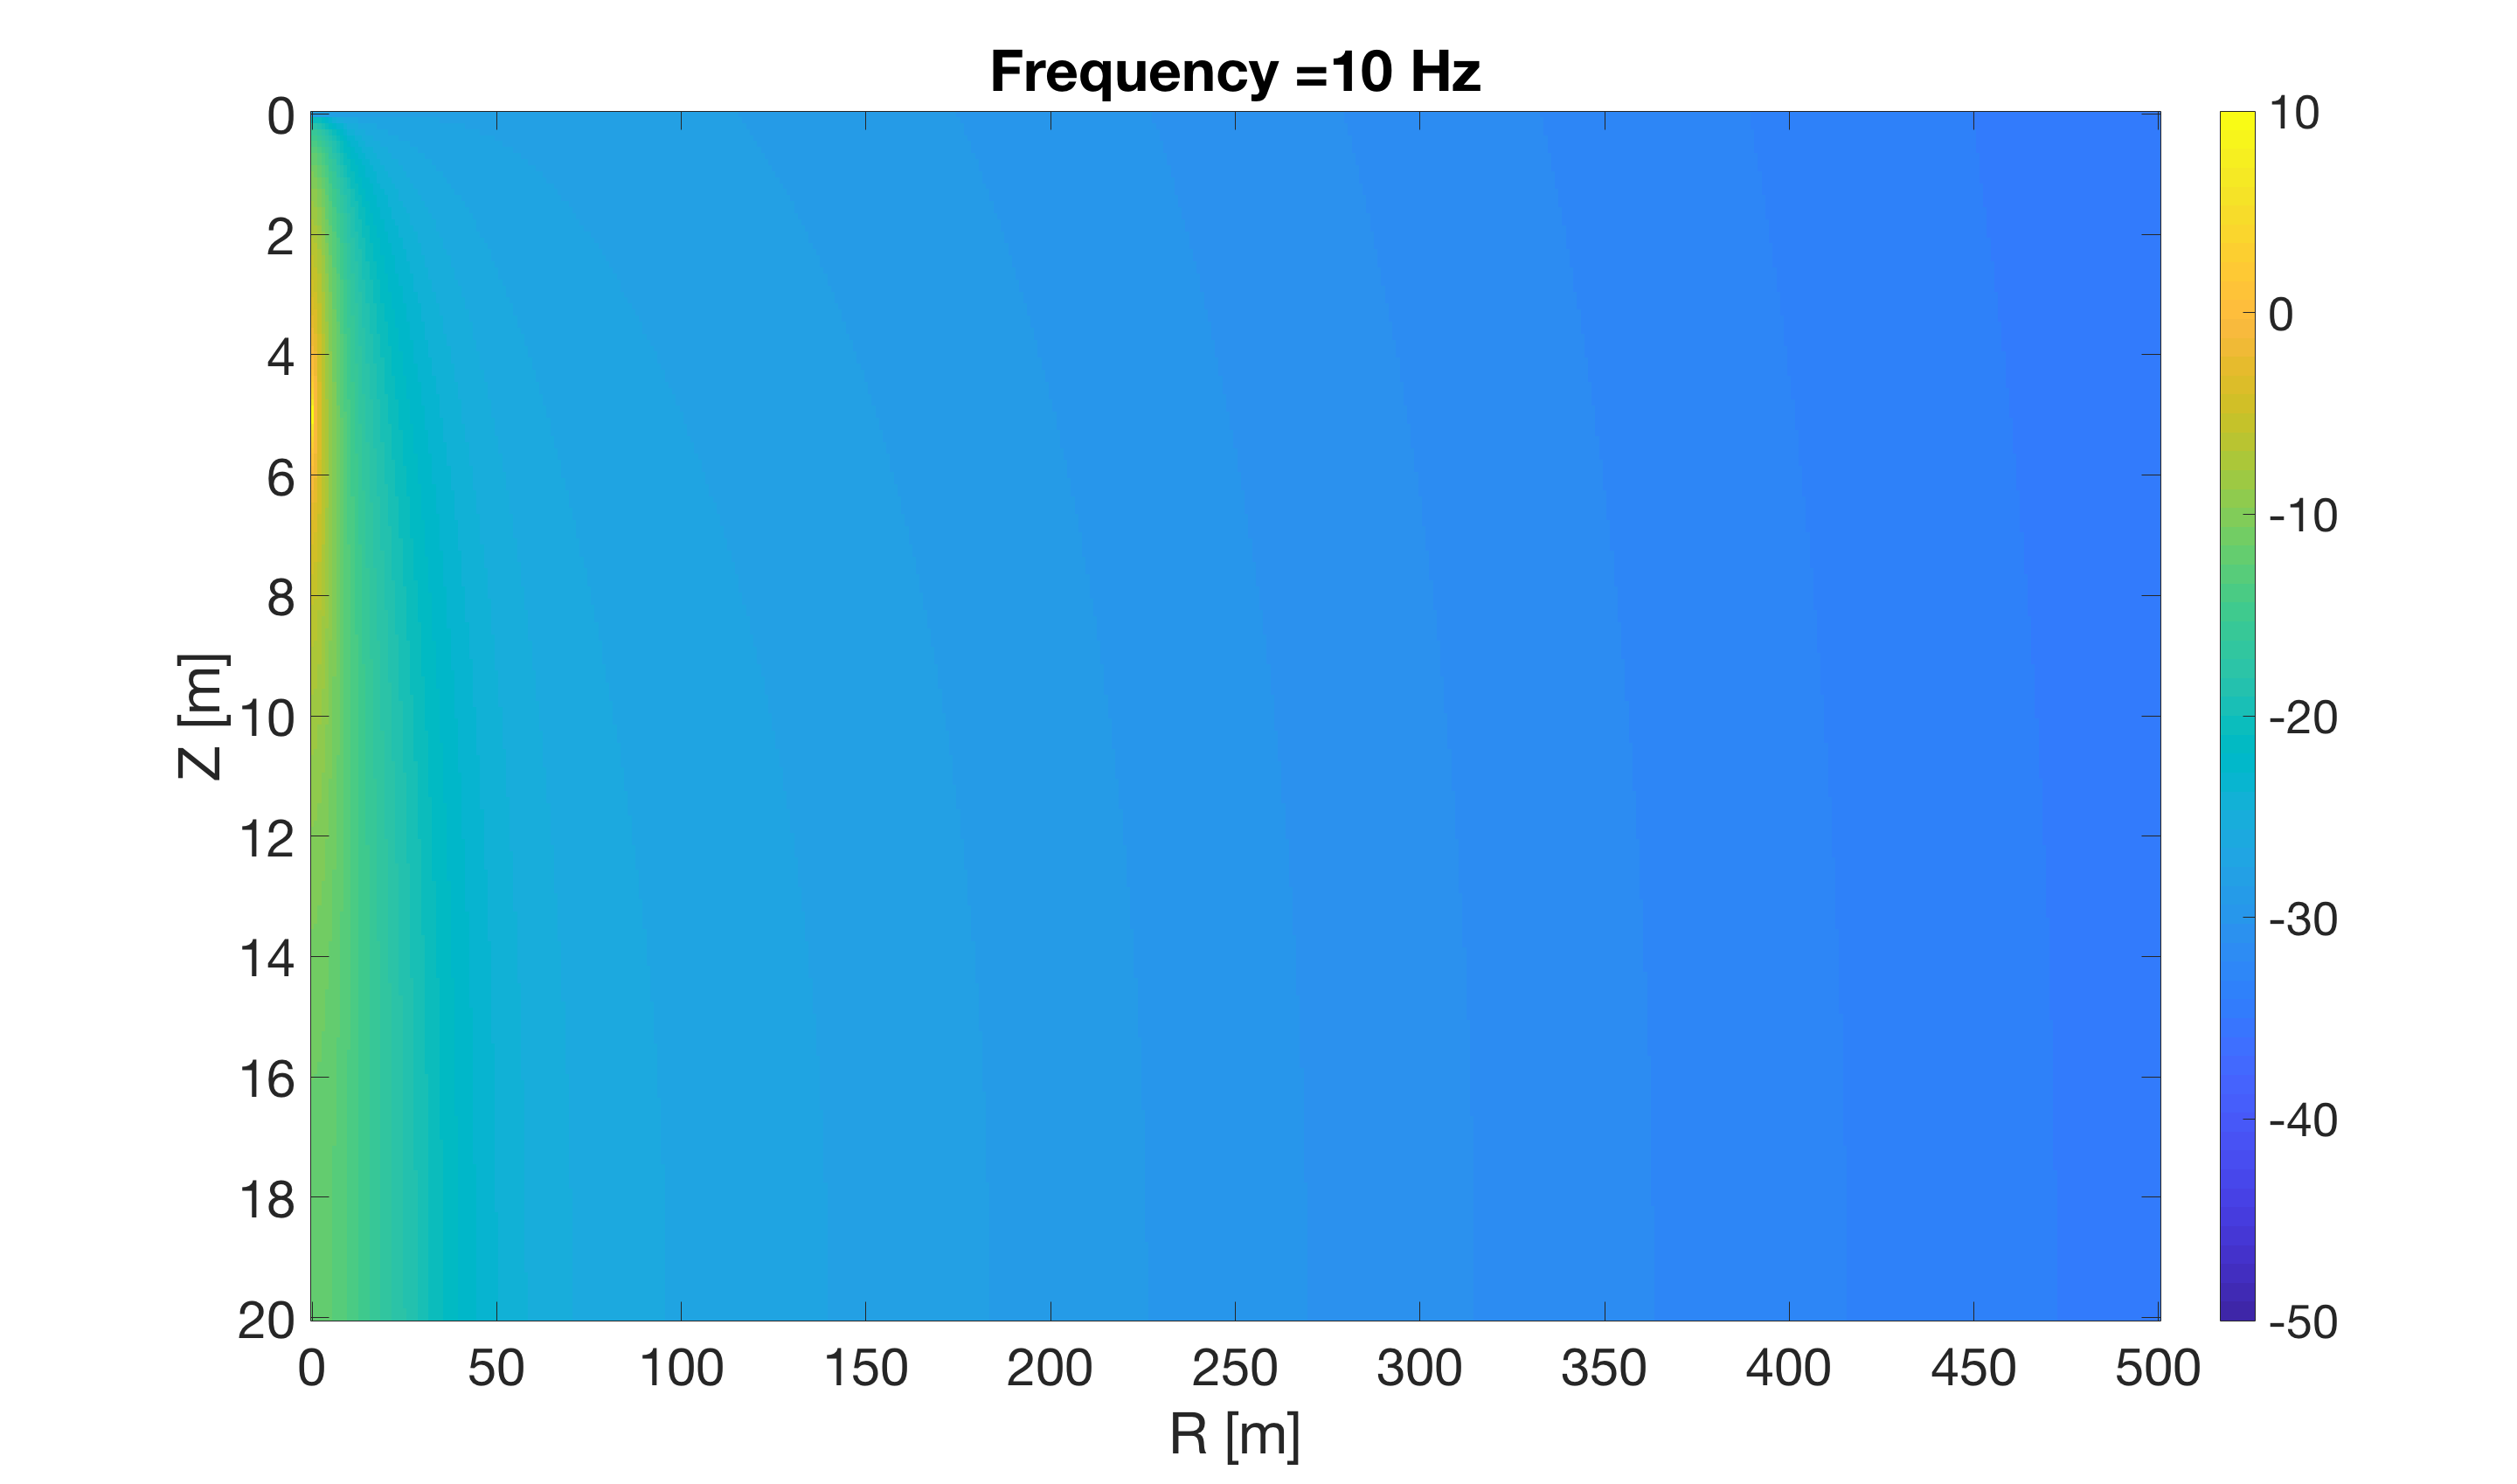
\includegraphics[width=95mm]{usp6_1.png}
}
\subfloat[Frequency, $\textit{f} = 100 Hz$]{
  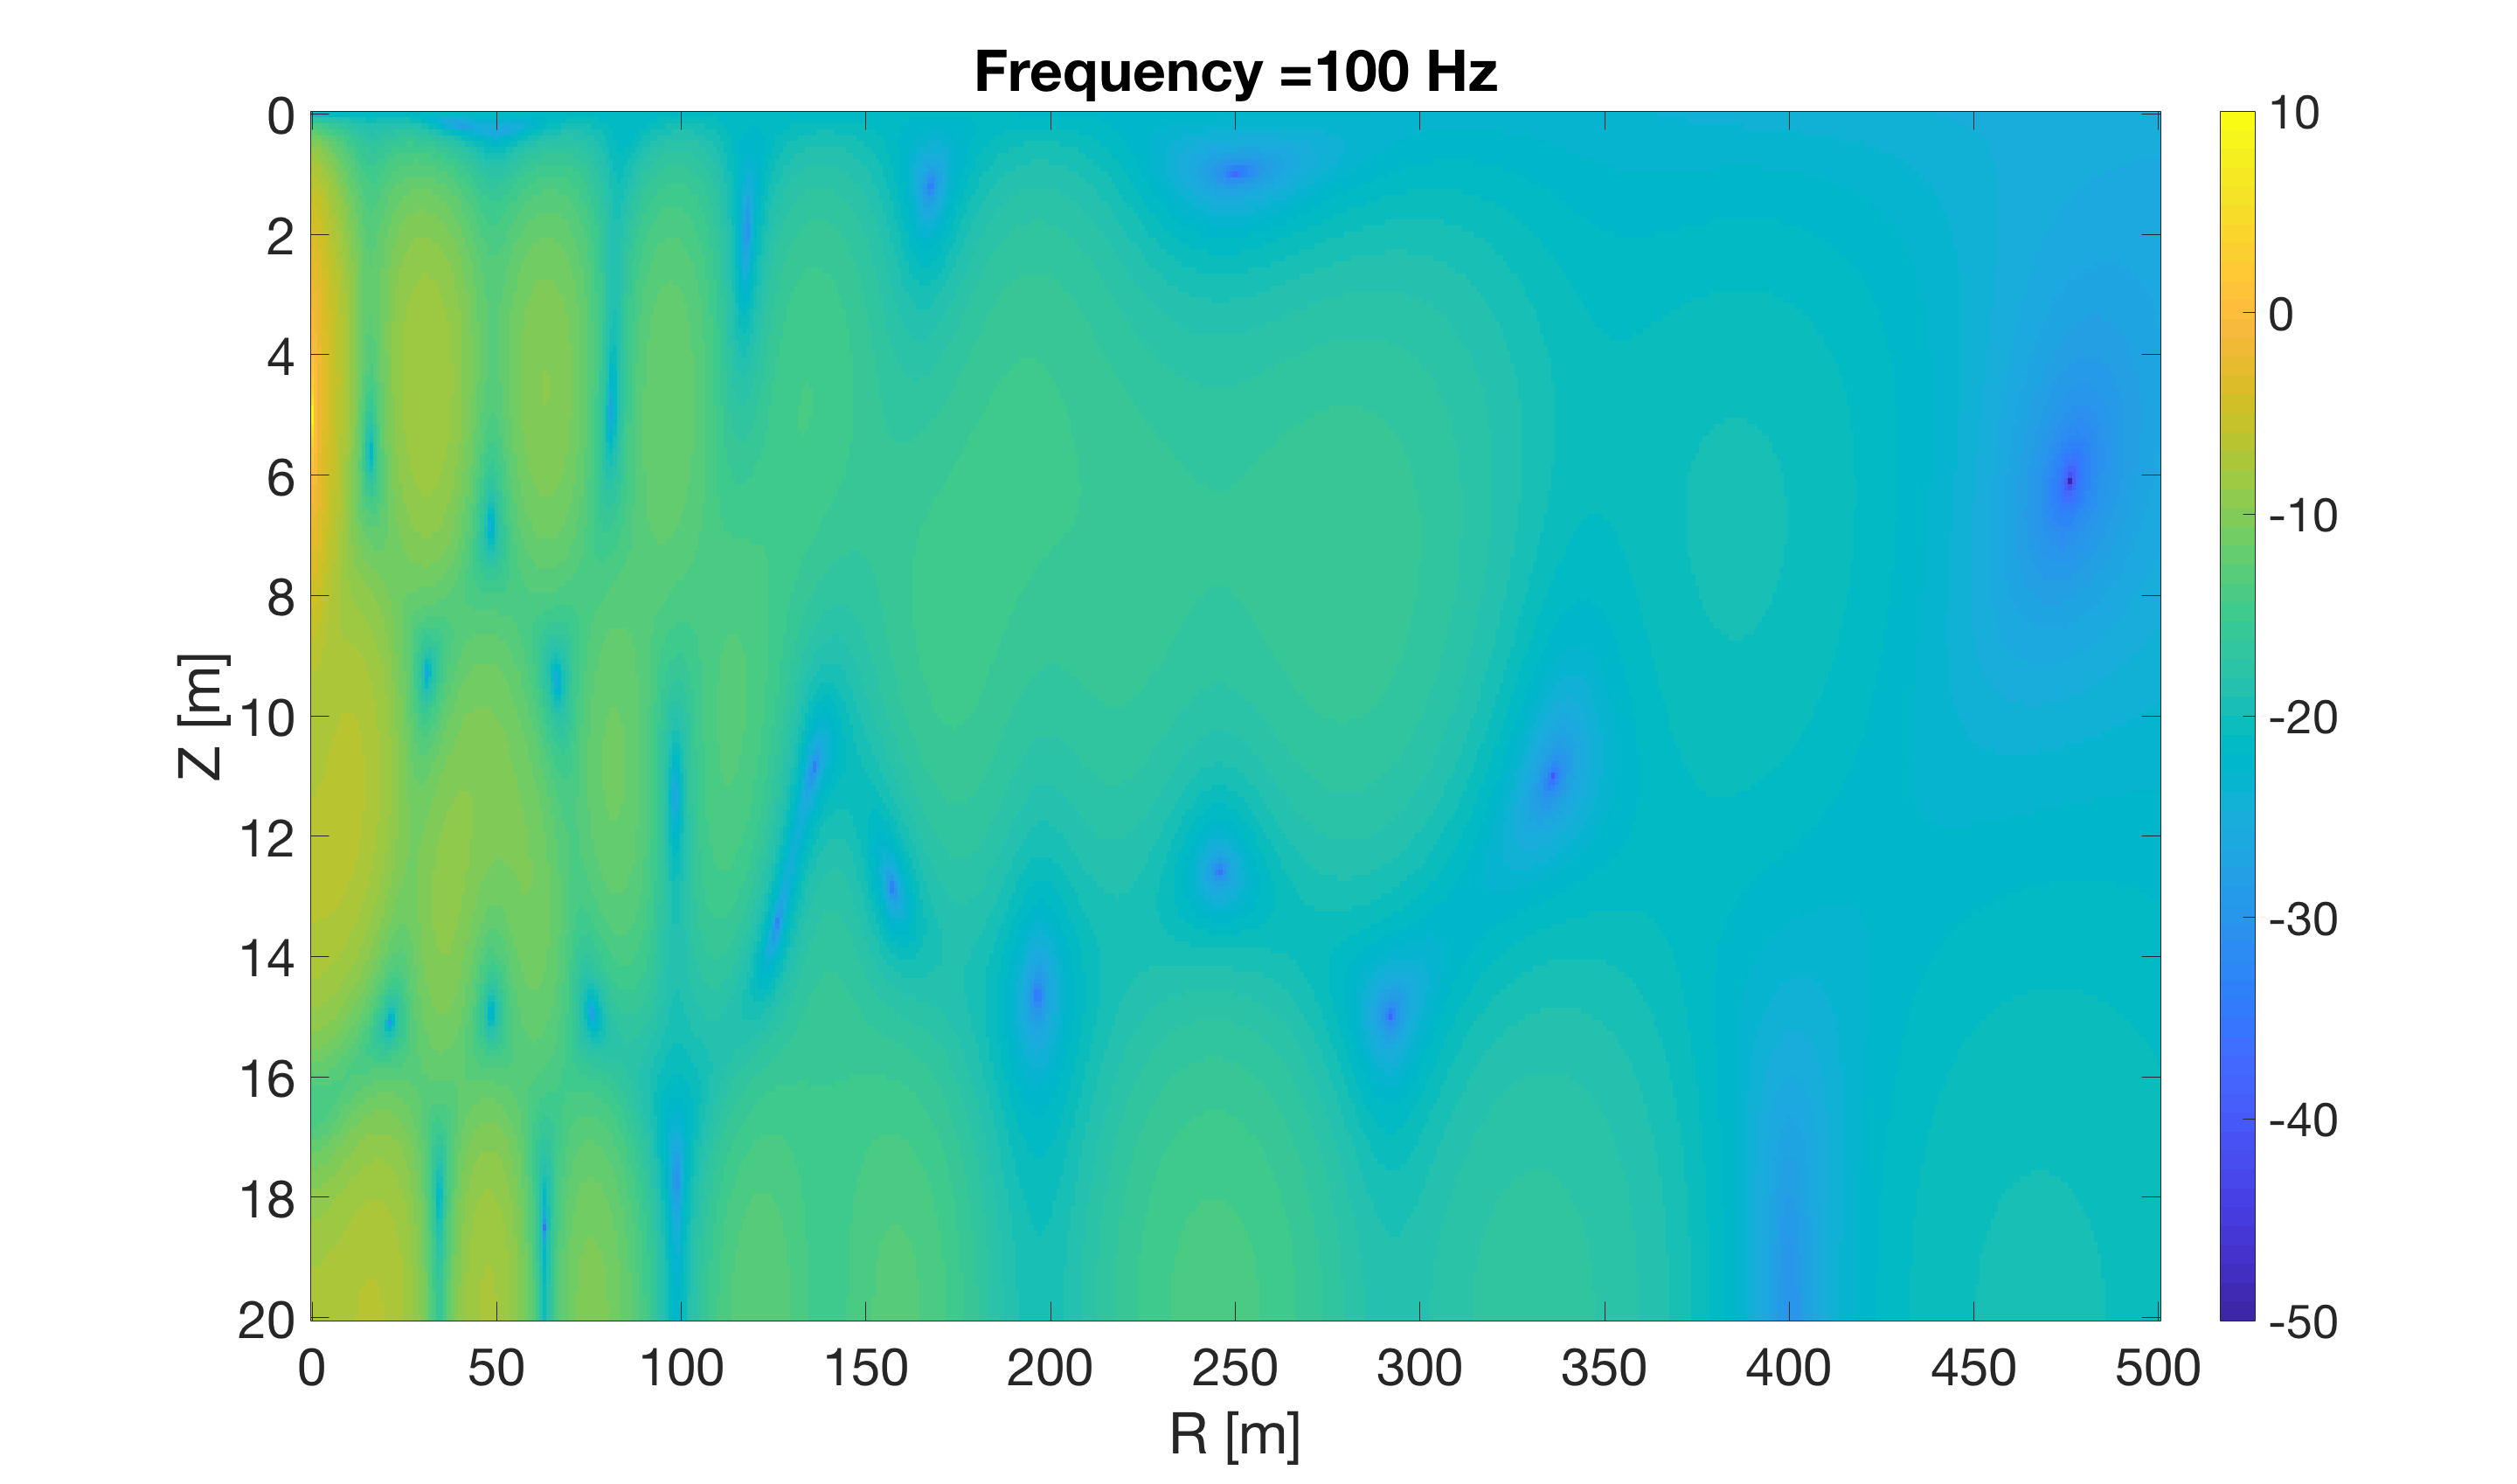
\includegraphics[width=95mm]{usp6_2.png}
}
\newline
\subfloat[Frequency, $\textit{f} = 1 kHz$]{
  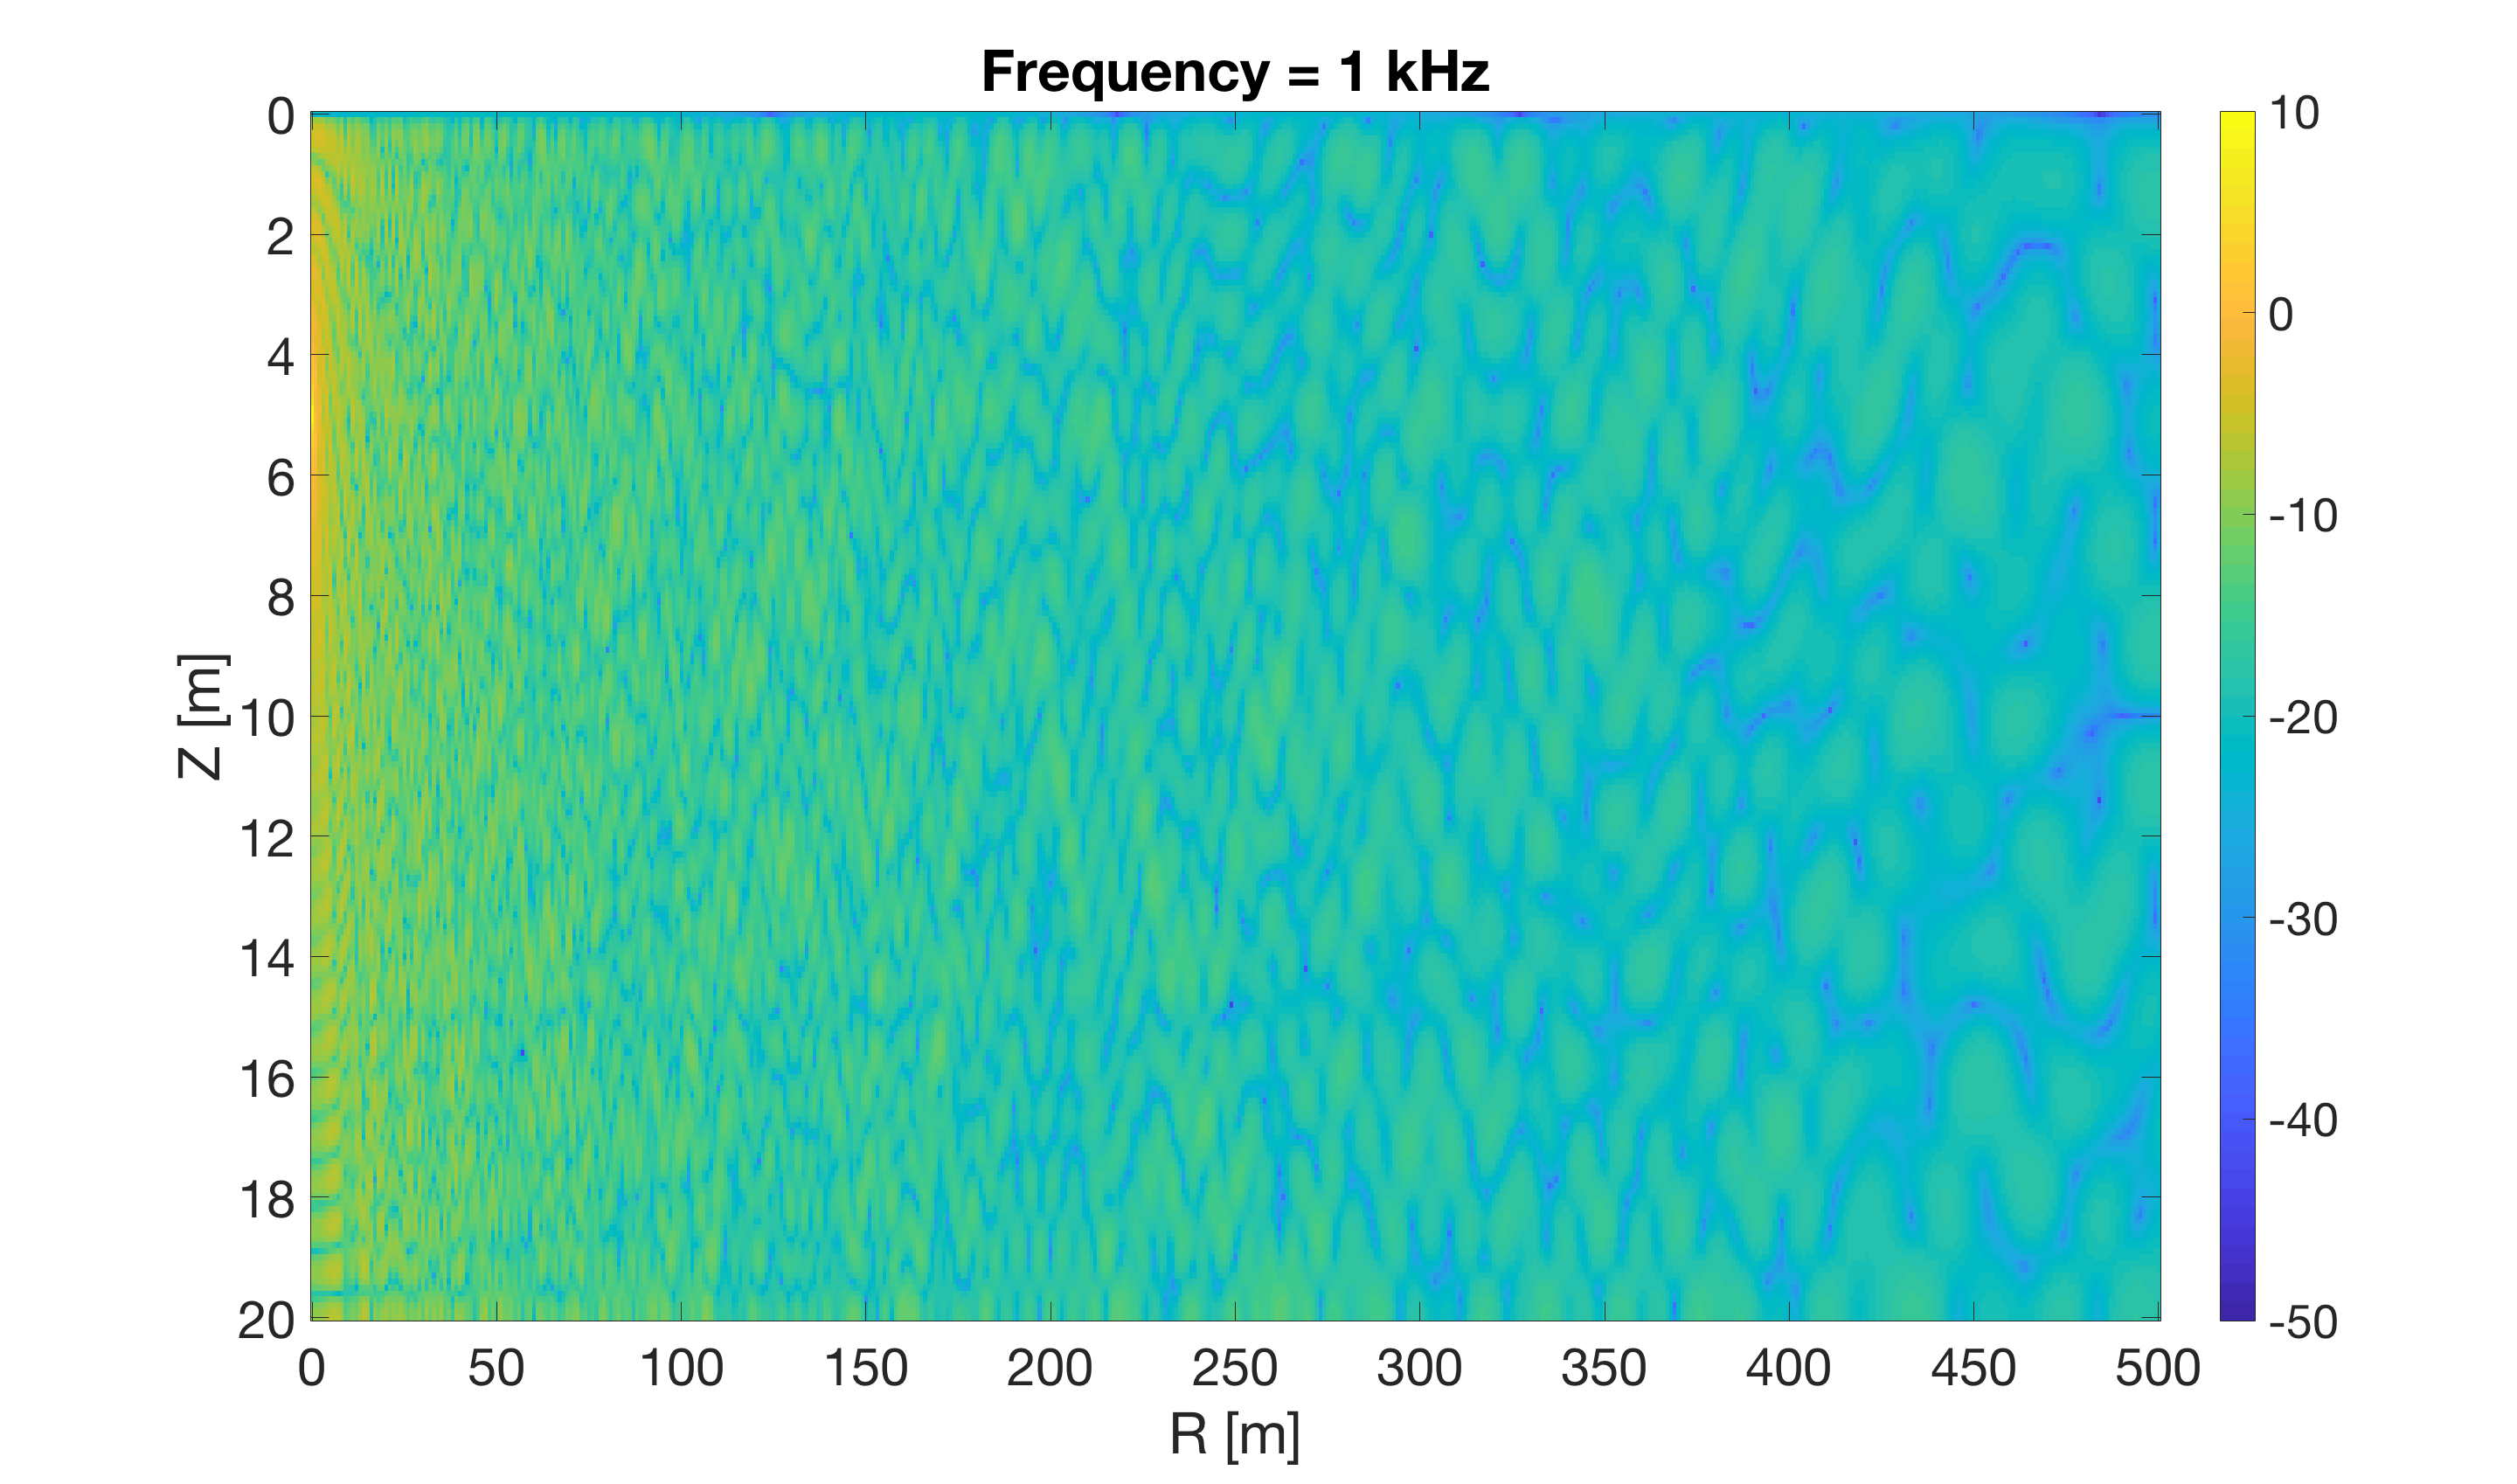
\includegraphics[width=95mm]{usp6_3.png}
}
\subfloat[Frequency, $\textit{f} = 10 kHz$]{
  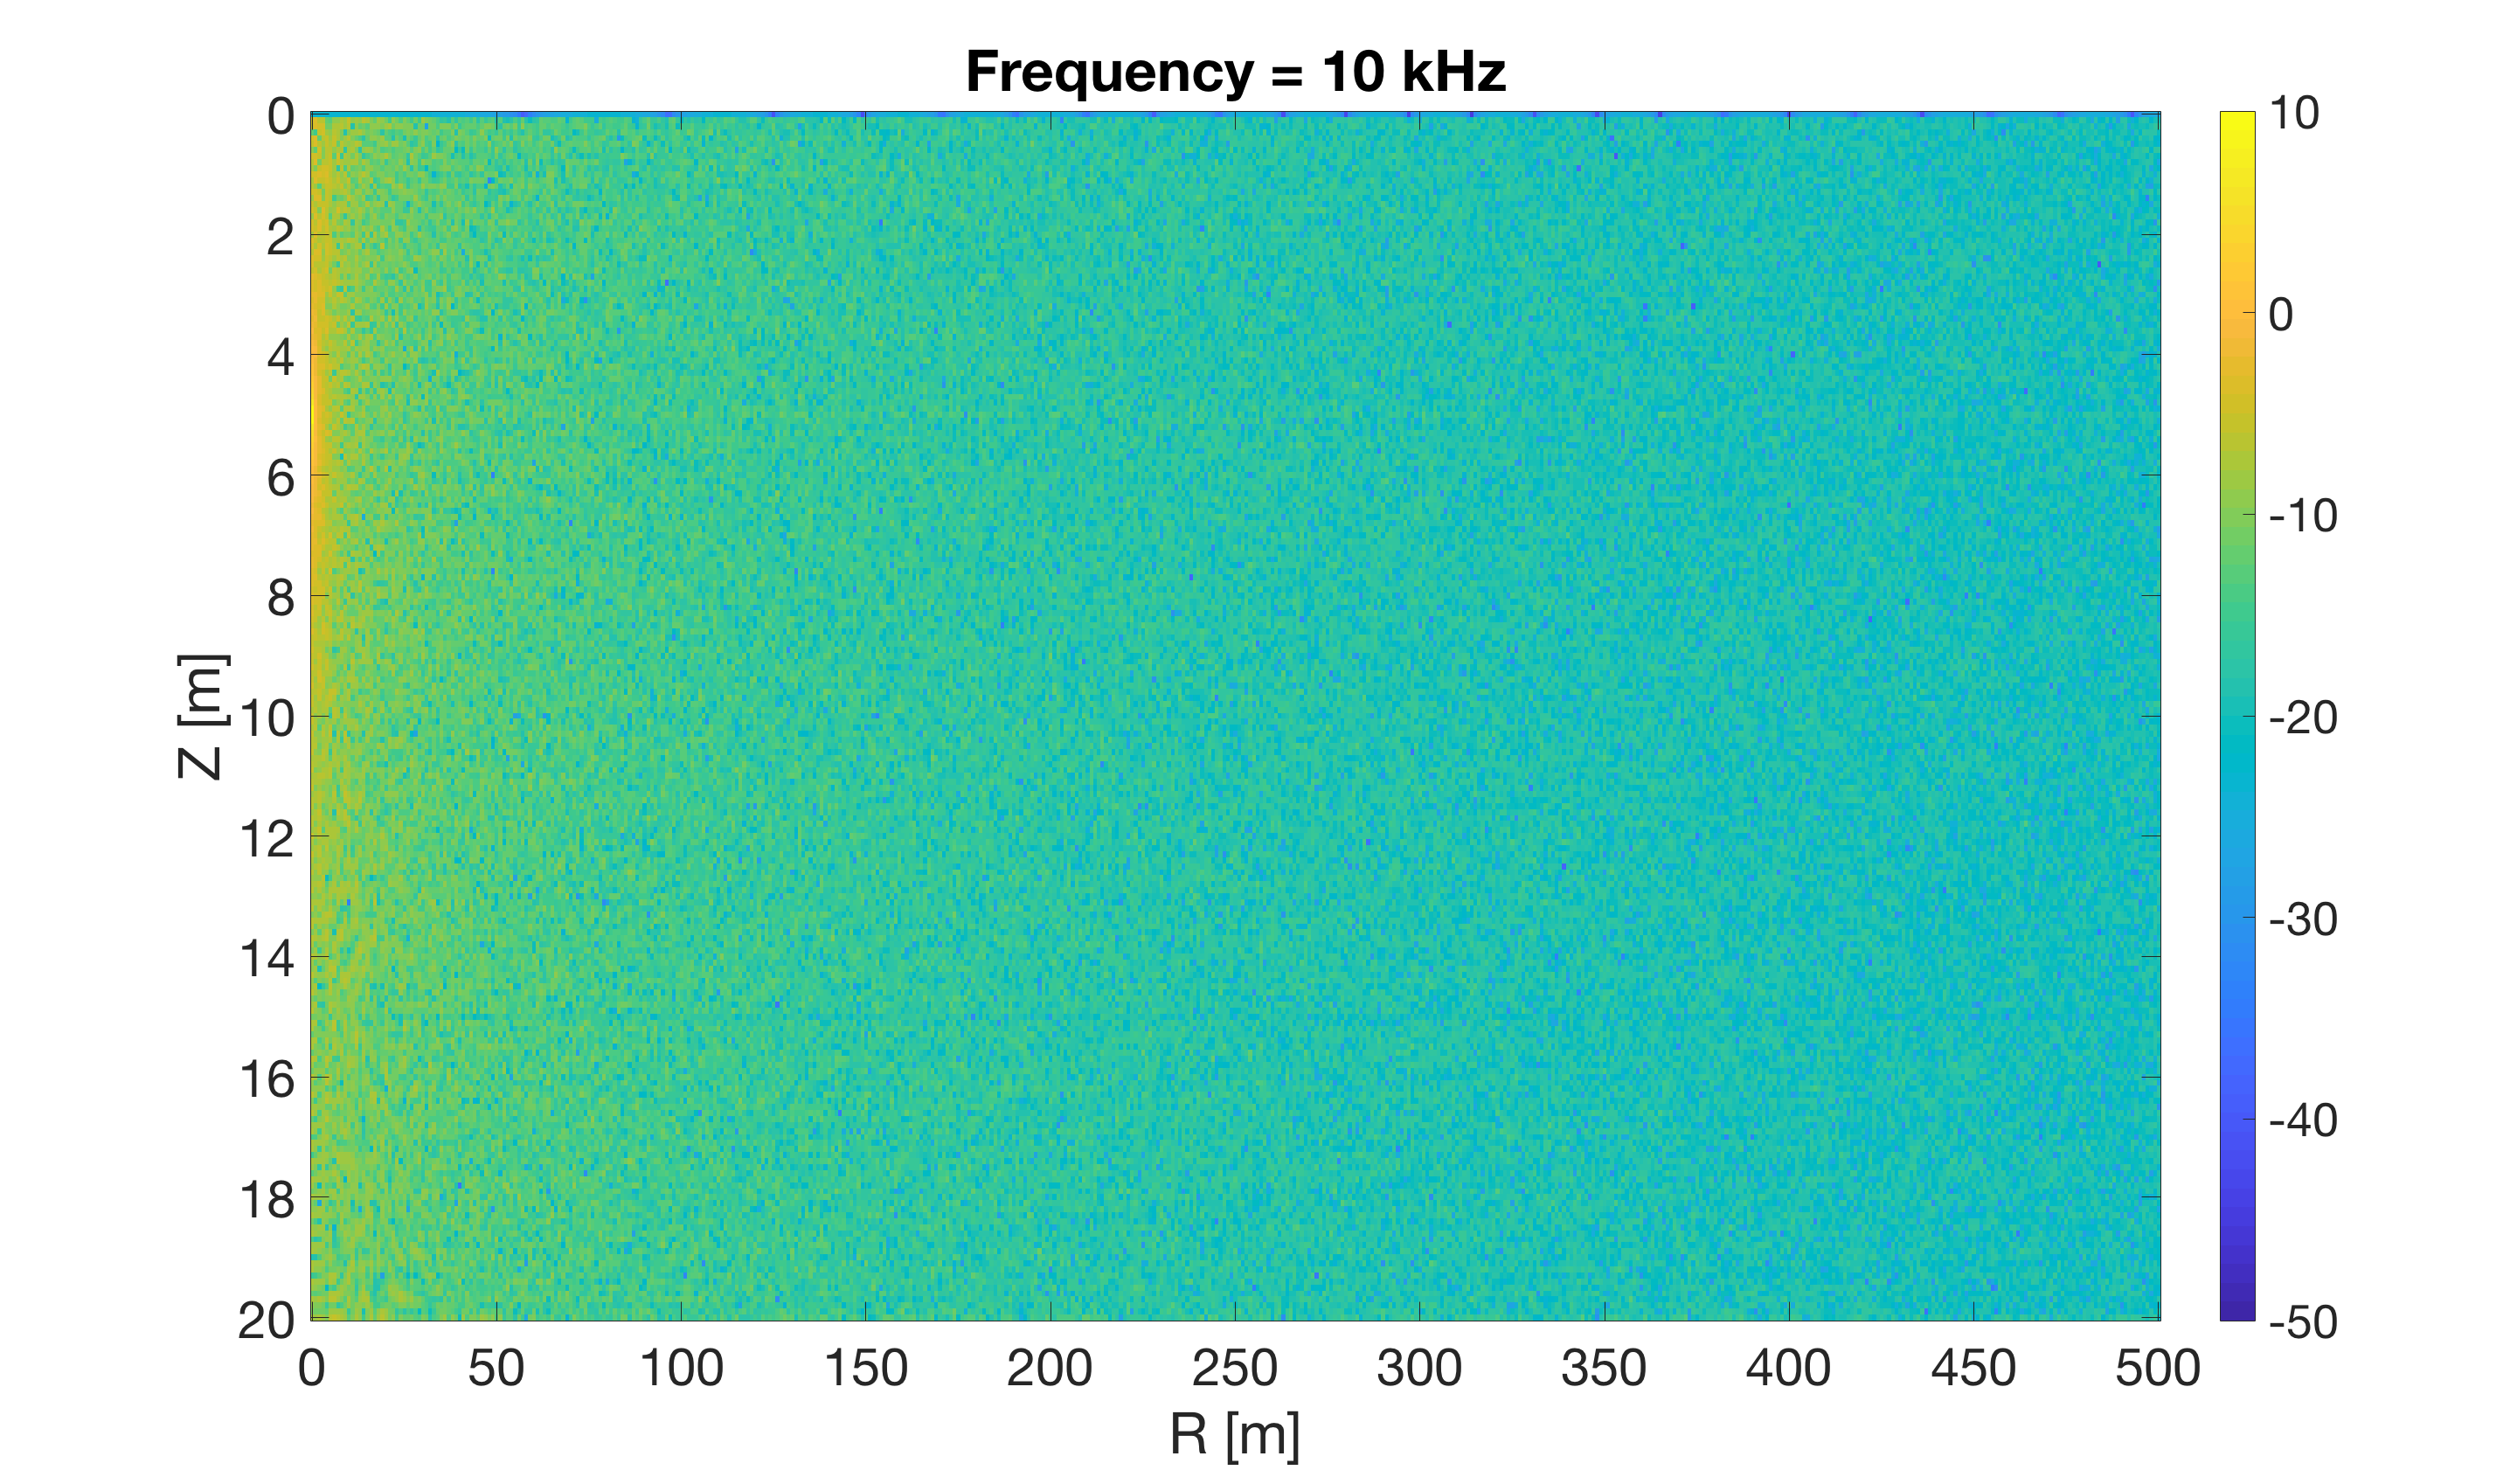
\includegraphics[width=95mm]{usp6_4.png}
}
\newline
\hbox to 18.5mm{}% !!
\subfloat[Frequency, $\textit{f} = 100 kHz$]{
  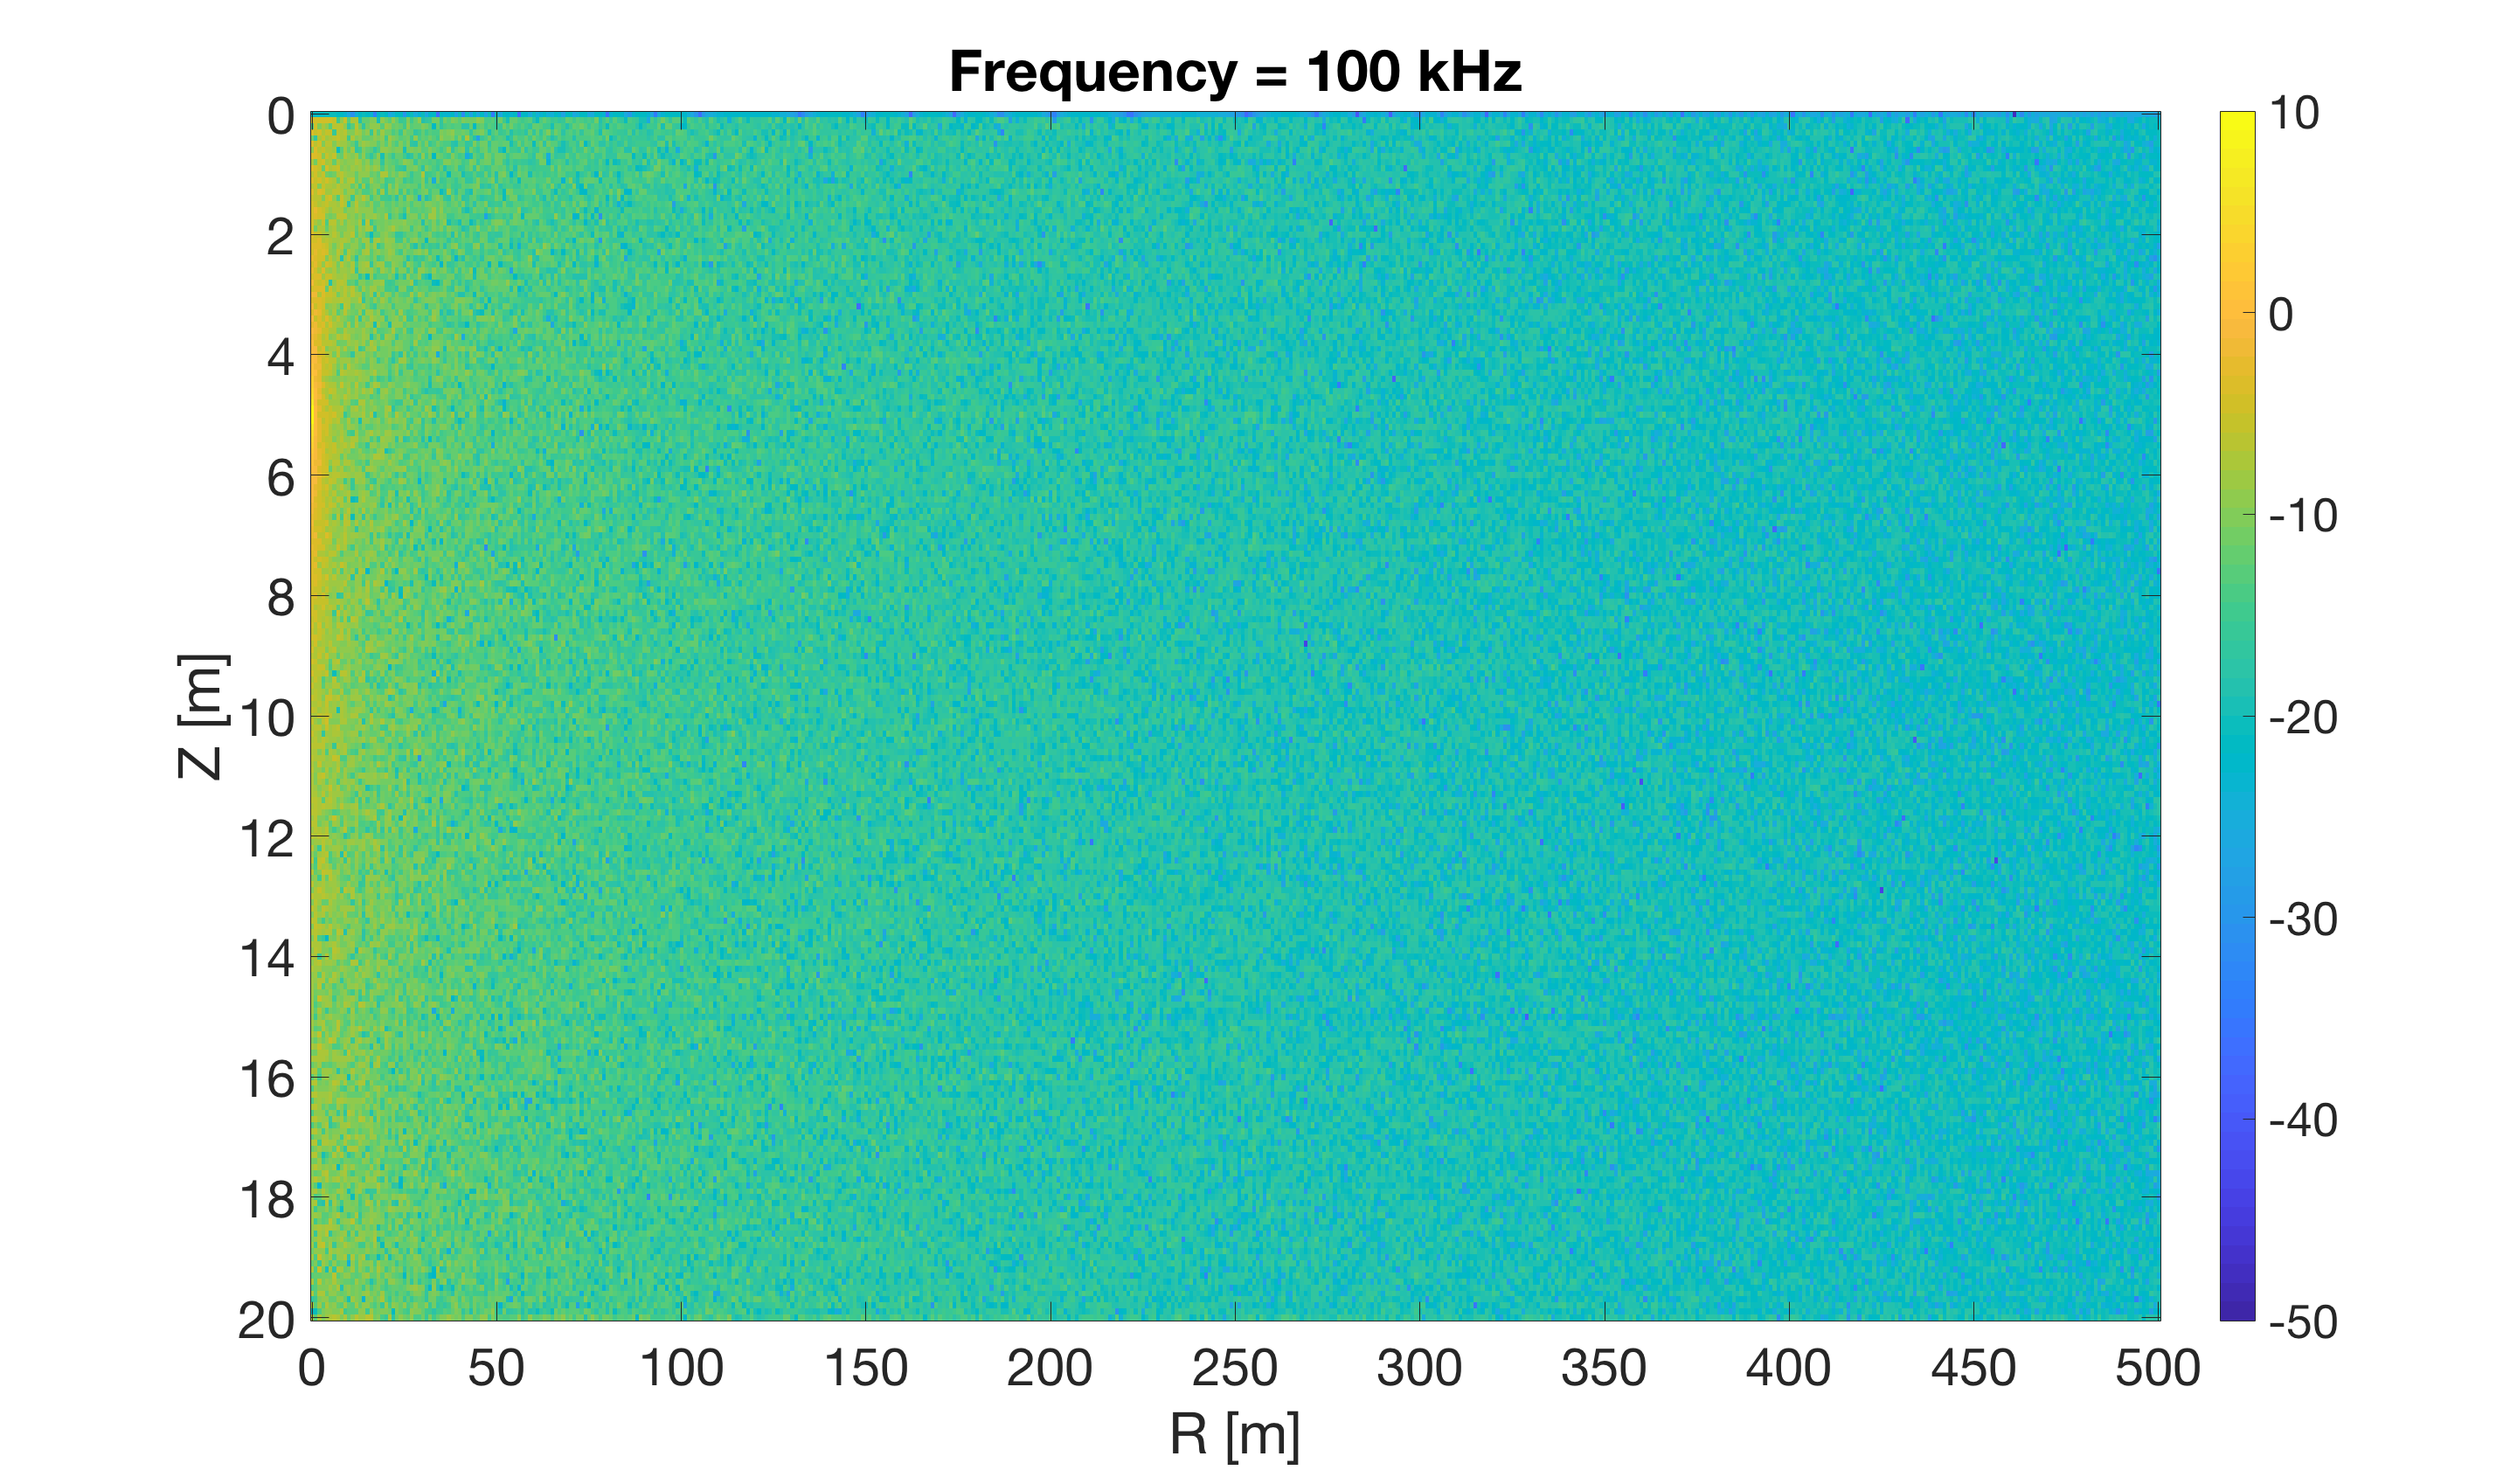
\includegraphics[width=90mm]{usp6_5.png}
}
\caption{ Pressure distribution observed at various frequencies }
\end{figure}




